\section{多元t分布}
\label{sec:mvd-t}

多元高斯的尾部很轻：传感器例子中，读数偏离均值超过三个标准差的机会只有千分之几。可是实际环境有时整体变得嘈杂，比如房间的空调启动，两台传感器的误差同时放大。这种“整体波动”不是加在某一台上的独立扰动，而是一个乘在所有分量上的共同尺度。

把多元高斯中固定的尺度换成随机的共同尺度，就得到多元t分布。本节先构造它并求出联合密度，再弄清位置、尺度矩阵和自由度三种参数的不同作用，最后说明共同尺度造成的依赖：即使尺度矩阵是对角的，分量也不独立。

一元情形已在第~\ref{chap:common-distributions}章出现：位置为$\mu$、尺度为$s>0$、自由度为$\nu>0$的t分布密度是
\[
 f(x)=\frac{\Gamma\bigl(\frac{\nu+1}{2}\bigr)}{\Gamma\bigl(\frac{\nu}{2}\bigr)\sqrt{\nu\pi}\,s}\Bigl(1+\frac{(x-\mu)^{2}}{\nu s^{2}}\Bigr)^{-(\nu+1)/2} ,
\]
$\nu=1$时就是Cauchy分布。下面的构造在$d=1$时回到它。

\subsection{正态尺度混合}
\label{sec:mvd-t-mixture}

\paragraph{构造}
取一个高斯向量和一个控制尺度的正随机变量，两者独立，用后者统一放大前者。为使结果的边缘回到一元t分布，尺度取为$\chi^2$变量倒数的平方根。

\begin{definition}[多元t分布]
\label{def:mvd-t}
设$\nu>0$，$\bm{\mu}\in\mathbb{R}^{d}$，$\bm{\Sigma}$是$d\times d$正定矩阵。$\bm{Z}\sim\mathcal{N}(\bm{0},\bm{\Sigma})$与$U\sim\chi^2_\nu$相互独立，令
\begin{equation}
 \bm{X}=\bm{\mu}+\sqrt{\nu/U}\,\bm{Z} .
 \label{eq:mvd-t-construction}
\end{equation}
称$\bm{X}$服从位置为$\bm{\mu}$、\term{尺度矩阵}（scale matrix）为$\bm{\Sigma}$、自由度为$\nu$的\term{多元t分布}（multivariate t distribution）。
\end{definition}

记$V=\sqrt{\nu/U}$。它对所有分量相同：$\bm{X}-\bm{\mu}=V\bm{Z}$的每个分量都乘以同一个$V$。这种把高斯向量乘上一个独立随机尺度的构造称为\term{正态尺度混合}（normal scale mixture）：固定$U=u$，$\bm{X}=\bm{\mu}+\sqrt{\nu/u}\,\bm{Z}$，由式~\eqref{eq:mvd-gaussian-affine}，
\[
 \bm{X}\text{在}U=u\text{时服从}\ \mathcal{N}\Bigl(\bm{\mu},\ \frac{\nu}{u}\bm{\Sigma}\Bigr) .
\]
$\bm{X}$的分布就是这些高斯分布按$U$的分布加权混合。

$U$的均值是$\nu$，所以$V$大致在$1$附近，但$U$可以很接近$0$，此时$V$很大，整个向量被大幅放大。图~\ref{fig:mvd-t-scale}(a)画出不同自由度下$V$的密度：$\nu=1$时$V$有很长的右尾，$\nu=30$时$V$已经紧紧围着$1$。

\paragraph{联合密度}
因为$\bm{Z}$与$U$独立，$(\bm{Z},U)$的联合密度是两者密度之积。对区域$S$，先对$\bm{z}$积分、再对$u$积分，
\[
 \mathbb{P}(\bm{X}\in S)=\int_0^{\infty}f_U(u)\,\mathbb{P}\Bigl(\bm{\mu}+\sqrt{\nu/u}\,\bm{Z}\in S\Bigr)\,\mathrm{d}u .
\]
括号里的概率是$\mathcal{N}(\bm{\mu},(\nu/u)\bm{\Sigma})$的密度在$S$上的积分。被积函数非负，可以交换两次积分的次序，于是$\bm{X}$有密度
\begin{equation}
 f_{\bm{X}}(\bm{x})=\int_0^{\infty}f_U(u)\,g_u(\bm{x})\,\mathrm{d}u ,
 \label{eq:mvd-scale-mixture-density}
\end{equation}
其中$g_u$是$\mathcal{N}(\bm{\mu},(\nu/u)\bm{\Sigma})$的密度。式~\eqref{eq:mvd-scale-mixture-density}对任何独立的正尺度都成立，下一节的多元Laplace分布也用它。

\begin{theorem}[多元t密度]
\label{thm:mvd-t-density}
定义~\ref{def:mvd-t}中的$\bm{X}$有联合密度
\begin{equation}
 f_{\bm{X}}(\bm{x})=\frac{\Gamma\bigl(\frac{\nu+d}{2}\bigr)}{\Gamma\bigl(\frac{\nu}{2}\bigr)(\nu\pi)^{d/2}(\det\bm{\Sigma})^{1/2}}\Bigl(1+\frac{Q(\bm{x})}{\nu}\Bigr)^{-(\nu+d)/2},
 \label{eq:mvd-t-density}
\end{equation}
其中$Q$由式~\eqref{eq:mvd-gaussian-quadratic}给出。
\end{theorem}

\begin{proof}
把$\bm{\Sigma}$换成$(\nu/u)\bm{\Sigma}$，式~\eqref{eq:mvd-gaussian-density}给出
\[
 g_u(\bm{x})=\frac{u^{d/2}}{(2\pi\nu)^{d/2}(\det\bm{\Sigma})^{1/2}}\exp\Bigl(-\frac{uQ}{2\nu}\Bigr) .
\]
$\chi^2_\nu=\operatorname{Gamma}(\nu/2,1/2)$，其密度为
\[
 f_U(u)=\frac{u^{\nu/2-1}\mathrm{e}^{-u/2}}{2^{\nu/2}\Gamma(\nu/2)},\qquad u>0 .
\]

两者相乘，$u$的幂次合并为$u^{(\nu+d)/2-1}$，指数合并为$-u(1+Q/\nu)/2$。由Gamma积分
\[
 \int_0^{\infty}u^{a-1}\mathrm{e}^{-bu}\,\mathrm{d}u=\Gamma(a)\,b^{-a},\qquad a,b>0,
\]
取$a=(\nu+d)/2$，$b=(1+Q/\nu)/2$，
\[
 \int_0^{\infty}u^{\frac{\nu+d}{2}-1}\mathrm{e}^{-\frac{u}{2}(1+Q/\nu)}\,\mathrm{d}u=\Gamma\Bigl(\frac{\nu+d}{2}\Bigr)\,2^{(\nu+d)/2}\Bigl(1+\frac{Q}{\nu}\Bigr)^{-(\nu+d)/2} .
\]
最后整理常数：$2^{(\nu+d)/2}$与$f_U$中的$2^{-\nu/2}$合成$2^{d/2}$，再与$(2\pi\nu)^{-d/2}$合成$(\nu\pi)^{-d/2}$。
\end{proof}

$d=1$、$\bm{\Sigma}=s^{2}$时，$Q=(x-\mu)^{2}/s^{2}$，式~\eqref{eq:mvd-t-density}就是本节开头的一元t密度。与高斯一样，密度只通过$Q$依赖$\bm{x}$，等密度面仍是以$\bm{\mu}$为中心、由$\bm{\Sigma}$决定形状的椭球；这类分布称为\term{椭圆分布}（elliptical distribution）。不同的是密度沿椭球向外的衰减方式：高斯是$\mathrm{e}^{-Q/2}$，t是$Q$的负幂。

取$d=2$、$\nu=5$、$\bm{\mu}=\bm{0}$、$\bm{\Sigma}=\bm{I}$，由$\Gamma(3.5)=2.5\,\Gamma(2.5)$，常数是
\[
 \frac{\Gamma(3.5)}{\Gamma(2.5)\cdot5\pi}=\frac{2.5}{5\pi}=\frac{1}{2\pi},
\]
中心密度恰好与二维标准高斯相同。在$Q=25$，也就是离中心$5$个单位处，两者分别是
\[
 \frac{1}{2\pi}\Bigl(1+\frac{25}{5}\Bigr)^{-7/2}\approx3.0\times10^{-4},\qquad \frac{1}{2\pi}\mathrm{e}^{-25/2}\approx5.9\times10^{-7} ,
\]
相差约$500$倍。

\begin{BookInlineFigure}
  \centering
  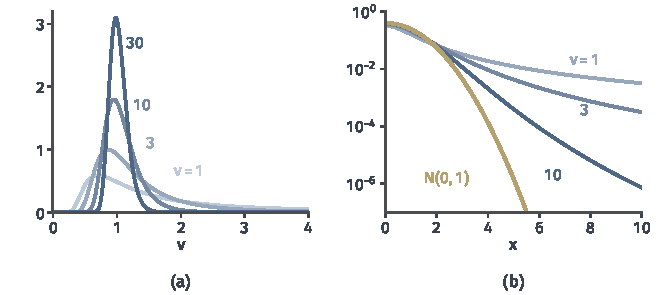
\includegraphics[width=112mm]{figures/07-probability/01-elementary-probability/matplotlib/mvd-t-scale/figure.pdf}
  \caption{共同尺度与尾部。(a)共同尺度$V=\sqrt{\nu/U}$的密度，$\nu=1,3,10,30$（蓝色由浅到深）；自由度越大，$V$越集中在$1$附近。(b)一个分量（$\Sigma_{i,i}=1$）的密度，纵轴取对数：t分布$\nu=1,3,10$（蓝色由浅到深）与$\mathcal{N}(0,1)$（黄）。}
  \label{fig:mvd-t-scale}
\end{BookInlineFigure}

\subsection{参数与矩}
\label{sec:mvd-t-moments}

\paragraph{位置与均值}
由构造，$\bm{X}-\bm{\mu}=V\bm{Z}$关于$\bm{\mu}$对称：$V\bm{Z}$与$-V\bm{Z}$同分布。所以$\bm{\mu}$总是分布的对称中心，也是每个分量的中位数。它是不是均值，要看$\bm{X}$的分量是否可积。

由$V$与$\bm{Z}$独立，
\[
 \mathbb{E}\lvert X_i-\mu_i\rvert=\mathbb{E}[V]\,\mathbb{E}\lvert Z_i\rvert ,
\]
而$\mathbb{E}\lvert Z_i\rvert$有限且为正。对$V$的矩，设$k\geq0$，由$U$的密度，
\[
 \mathbb{E}\bigl[U^{-k/2}\bigr]=\int_0^{\infty}\frac{u^{\nu/2-k/2-1}\mathrm{e}^{-u/2}}{2^{\nu/2}\Gamma(\nu/2)}\,\mathrm{d}u
\]
的有限性只取决于原点附近：积分在$0$附近收敛当且仅当$\nu/2-k/2>0$。

所以$\mathbb{E}[V^{k}]=\nu^{k/2}\mathbb{E}[U^{-k/2}]$在$k<\nu$时有限，在$k\geq\nu$时为无穷，从而
\[
 \mathbb{E}\lvert X_i-\mu_i\rvert^{k}<\infty\quad\Longleftrightarrow\quad k<\nu .
\]
特别地，$\nu>1$时均值存在，由$\mathbb{E}[\bm{Z}]=\bm{0}$，均值等于$\bm{\mu}$；$\nu\leq1$时均值不存在，$\bm{\mu}$只是位置。Cauchy情形$\nu=1$就是这样。

\paragraph{尺度矩阵与协方差}
$k=2$时，算出Gamma积分得
\[
 \mathbb{E}[1/U]=\frac{\Gamma(\nu/2-1)}{2\Gamma(\nu/2)}=\frac{1}{\nu-2},\qquad \nu>2 .
\]
于是$\nu>2$时
\begin{equation}
 \operatorname{Cov}(\bm{X})=\mathbb{E}[V^{2}]\,\operatorname{Cov}(\bm{Z})=\frac{\nu}{\nu-2}\,\bm{\Sigma} .
 \label{eq:mvd-t-cov}
\end{equation}
所以$\bm{\Sigma}$不是协方差矩阵，而是尺度矩阵：它决定椭球的形状和方向，协方差还要乘以共同尺度的二阶矩。两者只差一个正数倍，相关系数矩阵相同。

各种矩的存在条件按自由度列在表~\ref{tab:mvd-t-moments}中。

\begin{BookInlineTable}
  \centering
  \begin{tabular}{lcccc}
    \toprule
    自由度 & $0<\nu\leq1$ & $1<\nu\leq2$ & $2<\nu\leq4$ & $\nu>4$\\
    \midrule
    均值$\bm{\mu}$ & 不存在 & 存在 & 存在 & 存在\\
    协方差 & 不存在 & 不存在 & $\frac{\nu}{\nu-2}\bm{\Sigma}$ & $\frac{\nu}{\nu-2}\bm{\Sigma}$\\
    四阶矩 & 不存在 & 不存在 & 不存在 & 存在\\
    \bottomrule
  \end{tabular}
  \caption{多元t分布各阶矩的存在条件，“存在”指对应的期望有限。}
  \label{tab:mvd-t-moments}
\end{BookInlineTable}

\paragraph{边缘与线性组合}
取出第$i$个分量，$X_i=\mu_i+VZ_i$，$Z_i\sim\mathcal{N}(0,\Sigma_{i,i})$，$V$不变。这正是$d=1$时的同一构造，所以$X_i$服从位置$\mu_i$、尺度$\sqrt{\Sigma_{i,i}}$、自由度$\nu$的一元t分布。同理，$\bm{a}^{\top}\bm{X}$等于$\bm{a}^{\top}\bm{\mu}$加上$V\,\bm{a}^{\top}\bm{Z}$，服从尺度为$\sqrt{\bm{a}^{\top}\bm{\Sigma}\bm{a}}$的一元t分布，任意一组分量服从相应子矩阵的多元t分布。边缘与整体的自由度相同，因为它们共用同一个$U$。

一元t密度的尾部按$\lvert x\rvert^{-(\nu+1)}$衰减，所以$\nu$越小尾部越重，图~\ref{fig:mvd-t-scale}(b)。由上面的矩条件，这与“$k\geq\nu$阶矩不存在”是一回事：尾部太重，高阶矩积不出来。

\paragraph{自由度增大时}
$U\sim\chi^2_\nu$的均值为$\nu$、方差为$2\nu$，所以$U/\nu$的均值为$1$、方差为$2/\nu$。由第~\ref{chap:tail-probabilities}章的Chebyshev不等式，对任意$\varepsilon>0$，
\[
 \mathbb{P}\Bigl(\Bigl\lvert\frac{U}{\nu}-1\Bigr\rvert\geq\varepsilon\Bigr)\leq\frac{2}{\nu\varepsilon^{2}} .
\]
$\nu\to\infty$时右边趋于$0$，共同尺度$V=(U/\nu)^{-1/2}$越来越确定地接近$1$，$\bm{X}$也就越来越像$\mathcal{N}(\bm{\mu},\bm{\Sigma})$。从密度看，$(1+Q/\nu)^{-(\nu+d)/2}\to\mathrm{e}^{-Q/2}$，常数也趋于高斯的常数。$\nu$因此度量了“尺度有多不确定”：自由度小，尺度波动大，尾部重；自由度大，模型退回高斯。

\subsection{分量的依赖}
\label{sec:mvd-t-dependence}

设$\bm{\Sigma}$是对角矩阵，为简单起见取$\bm{\mu}=\bm{0}$、$\bm{\Sigma}=\bm{I}_d$。固定$U=u$时，$\bm{X}\sim\mathcal{N}(\bm{0},(\nu/u)\bm{I}_d)$，各分量相互独立：给定共同尺度，分量条件独立。$\nu>2$时由式~\eqref{eq:mvd-t-cov}，协方差矩阵也是对角的，分量两两不相关。可是不知道$U$的时候，一个分量很大，说明共同尺度可能很大，另一个分量也就更可能大。

\paragraph{联合密度不能分解}
先证明，对任何$\nu>0$，$d=2$时$X_1$与$X_2$不独立。若两者独立，对以$(x_1,x_2)$为中心、边长为$h$的小正方形，联合概率等于两个边长为$h$的区间概率之积。两边除以$h^{2}$，令$h\to0$，由三个密度的连续性得到
\[
 f_{\bm{X}}(x_1,x_2)=f_{X_1}(x_1)\,f_{X_2}(x_2)\qquad\text{对一切}(x_1,x_2) .
\]
于是对任意$a,b$，必须有
\[
 f_{\bm{X}}(a,b)\,f_{\bm{X}}(0,0)=f_{\bm{X}}(a,0)\,f_{\bm{X}}(0,b) ,
\]
因为两边都等于同样四个边缘密度值之积。

取$a=b=1$检验。由式~\eqref{eq:mvd-t-density}，$f_{\bm{X}}$与$k(Q)=(1+Q/\nu)^{-(\nu+2)/2}$成正比，上式要求$k(2)k(0)=k(1)^{2}$。但
\[
 \Bigl(1+\frac1\nu\Bigr)^{2}=1+\frac2\nu+\frac{1}{\nu^{2}}>1+\frac2\nu ,
\]
两边取$-(\nu+2)/2$次幂，不等号反向，得到$k(1)^{2}<k(2)=k(2)k(0)$。等式不成立，所以$X_1$与$X_2$不独立。

\paragraph{条件方差随观测增大}
依赖的方式可以算得很具体。固定$X_1=x_1$，把联合密度看成$x_2$的函数并提出与$x_2$无关的因子：
\[
 \Bigl(1+\frac{x_1^{2}+x_2^{2}}{\nu}\Bigr)^{-\frac{\nu+2}{2}}=\Bigl(1+\frac{x_1^{2}}{\nu}\Bigr)^{-\frac{\nu+2}{2}}\Bigl(1+\frac{x_2^{2}}{\nu+x_1^{2}}\Bigr)^{-\frac{\nu+2}{2}} .
\]
第二个因子正是自由度$\nu+1$、尺度$s$满足$(\nu+1)s^{2}=\nu+x_1^{2}$的一元t密度的形状。

所以给定$X_1=x_1$，$X_2$服从自由度$\nu+1$、尺度平方为$(\nu+x_1^{2})/(\nu+1)$的t分布。$\nu>1$时它的自由度大于$2$，由式~\eqref{eq:mvd-t-cov}的一元情形，
\begin{equation}
 \mathbb{E}[X_2^{2}\mid X_1=x_1]=\frac{\nu+x_1^{2}}{\nu+1}\cdot\frac{\nu+1}{\nu-1}=\frac{\nu+x_1^{2}}{\nu-1} .
 \label{eq:mvd-t-conditional-second-moment}
\end{equation}
它随$\lvert x_1\rvert$增大而增大。

取$\nu=5$：$X_2$的无条件方差是$5/3\approx1.67$；观测到$x_1=0$时条件二阶矩是$5/4=1.25$，观测到$x_1=3$时变为$14/4=3.5$。第一个分量平静，说明共同尺度多半不大，第二个分量也收敛一些；第一个分量剧烈，第二个分量的波动随之放大。图~\ref{fig:mvd-t-dependence}(b)用模拟样本核对了式~\eqref{eq:mvd-t-conditional-second-moment}。

\begin{BookInlineFigure}
  \centering
  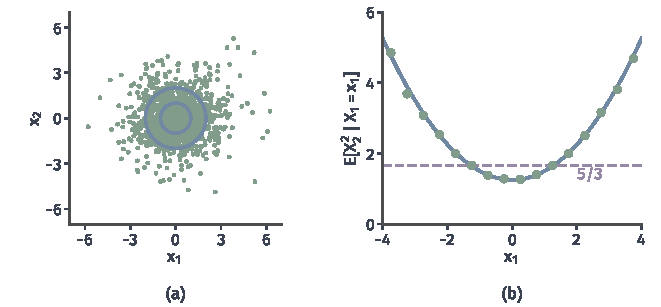
\includegraphics[width=112mm]{figures/07-probability/01-elementary-probability/matplotlib/mvd-t-dependence/figure.pdf}
  \caption{$\nu=5$、$\bm{\Sigma}=\bm{I}$的二维t分布，分量不相关但不独立。(a)$1500$个样本（绿，种子$31$）与等密度圆$Q=1,4$（蓝）；远处的点往往两个坐标同时偏大。(b)条件二阶矩$\mathbb{E}[X_2^{2}\mid X_1=x_1]=(5+x_1^{2})/4$（蓝），绿点是$40$万个样本（种子$32$）按$x_1$分组、组宽$0.5$的组内平均，紫色虚线是无条件方差$5/3$。}
  \label{fig:mvd-t-dependence}
\end{BookInlineFigure}

\paragraph{平方的协方差}
同样的依赖也能从矩看出来。$\nu>4$时$\mathbb{E}[1/U^{2}]=1/((\nu-2)(\nu-4))$，由$V$与$\bm{Z}$独立及$Z_1,Z_2$独立，
\[
 \mathbb{E}[X_1^{2}X_2^{2}]=\mathbb{E}[V^{4}]\,\mathbb{E}[Z_1^{2}]\,\mathbb{E}[Z_2^{2}]=\frac{\nu^{2}}{(\nu-2)(\nu-4)} .
\]
而$\mathbb{E}[X_1^{2}]$与$\mathbb{E}[X_2^{2}]$都等于$\nu/(\nu-2)$，两者之差为
\[
 \operatorname{Cov}(X_1^{2},X_2^{2})=\frac{2\nu^{2}}{(\nu-2)^{2}(\nu-4)}>0 .
\]
$\nu=5$时它等于$50/9\approx5.56$。$X_1$与$X_2$不相关，$X_1^{2}$与$X_2^{2}$却正相关：共同尺度让两个分量的大小一起涨落，而符号仍各自随机，所以线性的协方差看不到这种依赖。

如果想要“边缘是t分布、分量独立”的模型，就应让每个分量各用一个独立的尺度：$X_i=\mu_i+\sqrt{\nu/U_i}\,Z_i$，$U_1,\ldots,U_d$相互独立。它的边缘与多元t相同，协方差也相同，却是另一个联合分布，等密度线不再是椭圆。第~\ref{sec:mvd-comparison}节会比较两种模型在“同时出现大值”上的差别。
